\documentclass{beamer}
 
\usepackage[russian, french]{babel}
\usepackage[utf8]{inputenc}
\usepackage[T1]{fontenc}
\usepackage{amsmath}
\usetheme{Copenhagen}
\setbeamertemplate{navigation symbols}{}
%\title[Translittération automatique]{Données Séquentielles et Symboliques: Translittération automatique}
\title[Translittération automatique]{Données Séquentielles Symboliques: Translittération automatique}
\author[A.~Bérard, M.~Millet, C.~Robin]{Alexandre Bérard, Mathias Millet, Charles Robin}

\date{January 10th, 2014}

\newcommand*\oldmacro{}%
\let\oldmacro\insertshorttitle%
\renewcommand*\insertshorttitle{%
  \oldmacro\hfill%
  \insertframenumber\,/\,\inserttotalframenumber}

\begin{document}

\begin{frame}
\titlepage
\end{frame}

\begin{frame}{Sommaire}
  \tableofcontents
\end{frame}

\section{Introduction}   
 
\subsection{Translittération}
\begin{frame}
    \frametitle{Introduction: Translittération}
	%\framesubtitle{Translittération}
	\begin{block}{Definition}
	%Remplacement d'un graphème d'un système d'écriture par un ou plusieurs graphèmes d'un autre système d'écriture
        Conversion de texte d'un système d'écriture à un autre, en substitutant des \emph{graphèmes} ou des \emph{phonèmes}.
    \end{block}	    
    
	\begin{exampleblock}{Exemple: anglais - hindi}
	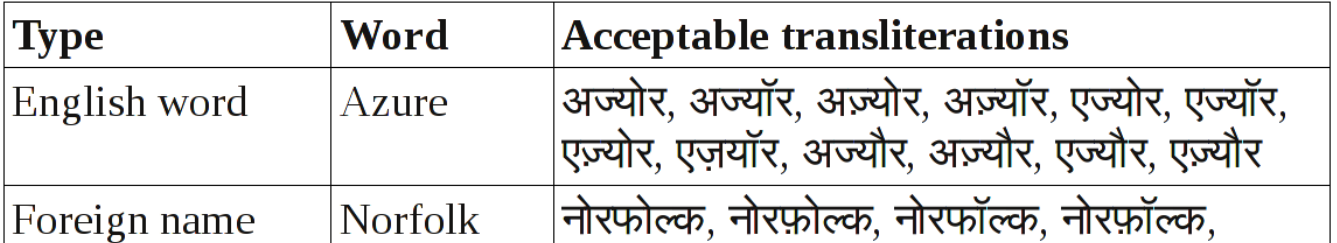
\includegraphics[scale=0.2]{en-in-example}
    \end{exampleblock}
    
	\begin{block}{Pourquoi ?}
	\begin{itemize}
		\item Traduction automatique de termes techniques, noms propres, ou requêtes Web.
		\item Plus besoin de maintenir un dictionnaire !
	\end{itemize}
	\end{block}	    
\end{frame}

\subsection{Le projet}


\begin{frame}
\frametitle{Introduction: le projet}
%\framesubtitle{Le projet}

	\begin{block}{L'objectif}
		Implémenter des techniques de translittération automatique
		\begin{itemize}
            \item De l'espagnol vers le portugais (\emph{SPA-POR})
            \item De l'anglais vers le russe (\emph{ENG-RUS})
		\end{itemize}
	\end{block}

	\begin{block}{Les données}
	Pour chaque paire de langages:		
		\begin{itemize}
            \item Un corpus d'apprentissage: 3057 entrées pour SPA-POR, et 7262 entrées pour ENG-RUS.
		\item Un corpus de test: 1000 entrées.
		\end{itemize}		
	\end{block}

\end{frame}

\begin{frame}[fragile]
\frametitle{Introduction: le projet : exemples}
\begin{block}{ENG-RUS}
\foreignlanguage{russian}{
\texttt{\#vitellin\# \#вителлин\# OR \#вителлины\#	other unknown}\\
\texttt{\#telephone\# \#телефон\# other unknown} }
\end{block}
\begin{block}{SPA-POR}
\texttt{\#teléfono\# \#telefone\#	other	unknown}\\
\texttt{\#thermosphaera\# \#thermosphaera\#	other	unknown}
\end{block}
\end{frame}


\subsection{Méthodologie}

\begin{frame}
\frametitle{Méthodologie}

	\begin{block}{Échantillonage?}
	Les données fournies sont déjà séparées entre données d'apprentissage et données de test\\
	$\Longrightarrow$ L'échantillonage n'est pas nécessaire
	\end{block}

	\begin{block}{Métriques}
	Deux métriques:
		\begin{itemize}
            \item Précision
            \item Distance de Levenshtein
		\end{itemize}		
	\end{block}
	
	\begin{alertblock}{}
	$\Longrightarrow$ Ces métriques seront utilisées tout au long du projet.
	\end{alertblock}	
	
\end{frame}

\section{Translittération}


\begin{frame}
\tableofcontents[currentsection, hideothersubsections]
\end{frame}



\subsection{Translittération par règles de substitution}

\begin{frame}[fragile]
	\frametitle{Espagnol - Portugais}

	\begin{block}{Premières considérations}
		\begin{itemize}
		\item Les deux langues sont très proches (51\% de précision sans rien faire)
		\item En appliquant les trois règles suivantes : {\scriptsize \begin{verbatim}
			is#->e#
			ción#->ção#
			ido#->ídeo#
			\end{verbatim}}
			nous obtenons 57\% de précision
		\end{itemize}
	\end{block}

	\begin{alertblock}{}
	$\Longrightarrow$ De bons résultat peuvent être obtenus en déterminant des règles automatiquement 
	\end{alertblock}
\end{frame}

\begin{frame}
	\frametitle{Apprentissage}

	\begin{block}{Objectif}
	Trouver un compromis entre :
		\begin{itemize}
		\item Fiabilité : la règle ne conduit pas à de fausses translittérations
		\item Généralisation : la règle peut s'appliquer à beaucoup de mots
		\end{itemize}			
	\end{block}

	\begin{alertblock}{}
	$\Longrightarrow$ Nous allons essayer de générer de règles en prenant ces deux paramètres en compte
	\end{alertblock}
\end{frame}

\begin{frame}[fragile]
\frametitle{Apprentissage}
\frametitle{Génération des règles}

	\begin{block}{Partie gauche :}
	 	\begin{itemize}
	 	\item Aligner les mots:
            {\scriptsize \begin{verbatim} [('#catars', '#catars'), ('is', 'e'), ('#', '#')] \end{verbatim}}
	 	\item Enumérer la liste des candidats de gauche, de longueur $\geq l$:
            {\scriptsize \begin{verbatim} ['is', 'sis', 'is#', 'sis#', ...] \end{verbatim}}
	 	\item Garder les candidats ayant un support suffisant :
            {\scriptsize \begin{verbatim} len([w for w in words if 'is' in w]) >= s \end{verbatim}}
		\end{itemize}
	\end{block}
	
	\begin{block}{Partie droite :}
        Prendre la partie droite de règle offrant le meilleur \emph{taux de confiance} ($\geq c$).
	\end{block}		
\end{frame}

\begin{frame}
\frametitle{Résultats}
\footnotesize
\begin{center}
\begin{tabular}{|c|c|c||c|c|c|}
\hline
Support $s$&Longueur $l$&Confiance $c$&Précision&Distance&Règles\\
\hline
2&6&0.80&56.8\%&0.82&104\\
\hline
2&5&0.80&\textbf{69.0\%}&\textbf{0.58}&315\\
\hline
2&4&0.80&68.1\%&0.59&584\\
\hline
\hline
3&5&0.80&67.3\%&0.61&195\\
\hline
5&5&0.80&67.2\%&0.61&\textbf{128}\\
\hline
1&5&0.80&64.5\%&0.68&1490\\
\hline
\hline
2&5&0.75&68.5\%&0.59&340\\
\hline
2&5&0.85&68.4\%&0.59&287\\
\hline
\end{tabular}
\end{center}
\normalsize
\end{frame}

\subsection{Traduction statistique}
\begin{frame}
\tableofcontents[currentsection]
\end{frame}
\begin{frame}
    \frametitle{Traduction statistique}
    \begin{figure}[H]
        \label{translation_alignment}
        %\caption{Traduction et translittération}
        \centering
        \vspace{0.3cm}
        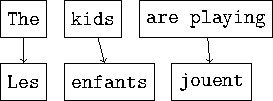
\includegraphics{word_alignment.pdf}
        \hspace{0.5cm}
        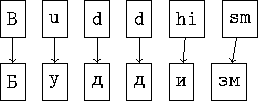
\includegraphics{letter_alignment.pdf}
    \end{figure}
\end{frame}

\subsection{CRF}

\begin{frame}
\frametitle{Présentation}
    \begin{block}{Équation principale des CRF}
        \begin{equation}
            p(\textbf{s}|\textbf{o}) = \frac{1}{Z_0}exp(\sum_{t=1}^T\sum_k \lambda_k f_k(...))
            \label{eqcrf}
        \end{equation}
    \end{block}
    \begin{figure}[H]
        \label{imagecrf}
        %\caption{Traduction et translittération}
        \centering
        \vspace{0.3cm}
        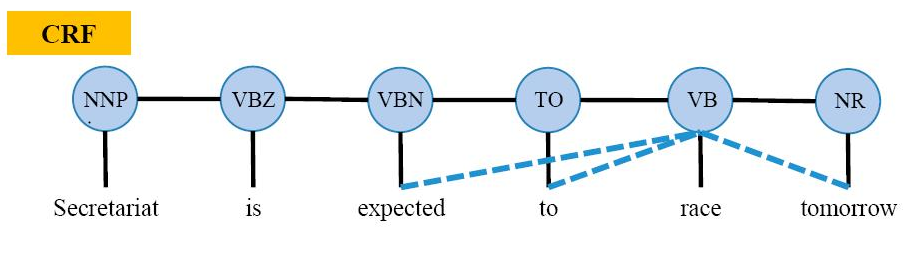
\includegraphics[width=\textwidth]{crf.png}
    \end{figure}

\end{frame}

\begin{frame}[fragile]
\frametitle{Champs conditonnels aléatoires}
	\begin{block}{Méthode}
		\begin{itemize}
		\item Alignement grâce à dpalign
		\item Utilisation de CRF++ :
		{\scriptsize \begin{verbatim}
		# Unigram
		U0:%x[0,0]
		U1:%x[-1,0]
		U2:%x[1,0]
		U3:%x[-2,0]
		U4:%x[2,0]
		U5:%x[-3,0]
		U6:%x[3,0]
		# Bigram
		B
		\end{verbatim}}
		\end{itemize}
	\end{block}
\end{frame}

\begin{frame}
\frametitle{Résultats}
\begin{block}{Résultats}
\begin{center}
\begin{table}[H]
\caption{Résultats pour le jeu de données \emph{Espagnol-Portugais} }
\begin{tabular}{|l|c|c|}
\hline
Règles&Précision&Distance d'édition\\
\hline
Baseline&51.0\%&1.06\\
\hline
3 subst.&58.6\%&0.76\\
\hline
CRF&\textbf{63.9\%}&\textbf{0.69}\\
\hline
\end{tabular}
\end{table}
\end{center}
\end{block}

\begin{block}{Résultats}
\begin{center}
\begin{table}[H]
\caption{Résultats pour le jeu de données \emph{Anglais-Russe} }
\begin{center}
\begin{tabular}{|c|c|}
\hline
Précision&Distance d'édition\\
\hline
49.8\%&1.61\\
\hline
\end{tabular}
\end{center}
\end{table}
\end{center}
\end{block}

\end{frame}

\section{Conclusion}
\begin{frame}
\tableofcontents[currentsection, hideothersubsections]
\end{frame}
\begin{frame}[allowframebreaks]
    \frametitle{Bibliography}
    {\fontsize{0.8em}{1em}
    \nocite{*}
    \bibliographystyle{plain}
    \bibliography{presentation}}
\end{frame}

\begin{frame}
    \frametitle{Conclusion}
    \begin{block}{}
    \begin{itemize}
        \item Possibilité d'optimiser le réglage des paramètres
        \item Bruit dans les données
        \item Approches futures: Étudier translittération inverse
    \end{itemize}
\end{block}
    \url{https://code.google.com/p/transliteration}
\end{frame}

\end{document}
